\documentclass[11pt,a4paper]{article}
 
\usepackage{polski}
\usepackage[utf8]{inputenc} %utf-8 żeby nie było problemów z przenoszeniem między windowsem a linuxem
\usepackage{graphicx}
\title{Generator raportów z bazy danych bazując na wzorcach}
\author{Maciej Kucharski}
\date{Semetr 13Z}
 
\begin{document}
\maketitle
 
% ogólna problematyka raportów
\section{Problematyka raportów}\label{sec:raport}
Raport to standardowa forma dokumentu biznesowego, który prezentuje informacje jakościowe i ilościowe w logiczny sposób. Raporty takie należą do jednych z najważniejszych dokumentów przedsiębiorstwa. Raport przedstawia widok informacji odpowiedni dla danej grupy odbiorców i powinien być automatycznie dostosowywany w zależności od użytkownika. Funkcje raportów to np.
ocena wydajności biznesowej, umożliwiająca szybkie sprawdzenie stanu oraz monitorowanie stopnia realizacji strategicznych celów przedsiębiorstwa, podsumowywanie kluczowych wskaźników biznesu, czy prezentacja miar biznesowych w oparciu o różne statystyki. W następnych punktach zostaną przedstawione najczęściej wykorzystywane wzorce raportów.
%master-detail
\subsection{Raport typu master-detail}\label{sec:master_detail}
Ten typ raportu prezentuje listę nadrzędnych wartości oraz szczegóły aktualnie wybranej pozycji. W zasadzie odpowiada strukturze typowego dokumentu, np. faktury. Idea pochodzi z lat 80-tych, kiedy to ekrany mieściły niewielką liczbę kolumn na raz, np. kilka podczas, gdy dane zawierały ich kilkanaście bądź kilkadziesiąt. W części nadrzędnej (master) prezentowane jest tylko kilka wspólnych kolumn, a w części podrzędnej (detail) wszystkie pozostałe pola. Jeśli raport jest prezentowany w sposób interaktywny, np. przez jakąś aplikację, część podrzędna jest "schowana" chyba, że użytkownik zarząda jej pokazania. Ten typ raportu może być zastosowany przy relacjach typu jeden-wiele. Zarówno obszar nadrzędny, jak i podrzędny może być formularzem, listą lub drzewem pozycji, co umożliwia wprowadzanie wielu stopni podrzędności, przy czym obszar podrzędny zwykle jest umieszczony pod lub obok obszaru nadrzędnego. Przykładem może być spis pozycji wchodzących w skład danego zamówienia lub działy przedsiębiorstwa wraz ze spisem pracowników każdego z nich.
%break groups
\subsection{Raporty z grupami łamiącymi (break groups)}\label{sec:break_groups}
Ten typ raportu polega na podziale wierszy trafiających do raportu na grupy o jednakowych wartościach w wyróżnionych kolumnach. Każdą z takich grup można odpowiednio obsłużyć, np. opatrywać je nagłówkami, czy wyliczać dla nich podsumowania. Taka struktura umożliwia dosyć elastyczną prezentację tych samych danych. Załóżmy, że mamy bazę pracowników zatrudnionych w różnych działach. Mogą oni być pogrupowani na podstawie działów, w których są zatrudnieni, następnie, w obrębie działów, można podzielić ich np. ze względu na lata pracy, a dodatkowo np. ze względu na przedziały ich zarobków. 
%macierzowy
\subsection{Raport macierzowy (krzyżowy)}\label{sec:macierzowy}
Raport macierzowy prezentuje związki między dwoma wymiarami. Takie raporty są często wykorzystywane przy różnego rodzaju ankietach. Prezentują związki między dwoma zmiennymi i ułatwiają znalezienie między nimi zależności. Struktura tego raportu przypomina arkusz kalkulacyjny programu Exel. Ułatwia to wspólne prezentacje danych, które pozornie nie mają ze sobą związku. Przykładem może być analiza ankiety, z której wynika na przykład, że pewien model samochodu sprzedaje się lepiej w pewnych województwach.
% raporty w Oracle XML Publisher
\section{Raporty w Oracle XML Publisher}\label{sec:raportOraclePublisher}
XML Publisher (zwany również BI Publisher) jest narzędziem umożliwiającym tworzenie raportów oraz zarządzanie nimi oraz ich dostarczanie. Ze względu na tematykę pracy, analizie będzie podlegać tylko pierwszy aspekt. Początkowo był fragmentem innego produktu Oracle, jednak od jakiegoś czas jest dostępny jako samodzielny program. Mimo bazowania na technologiach XSLT i XSL-FO nie jest zachowana pełna zgodność z W3C, jednak dla celów raportowania zapewnia wysoką wydajność i niezawodność. XML Publisher pozwala na tworzenie zaawansowanych raportów z użyciem XML jako formatu danych wejściowych. 

Narzędzie umożliwia tworzenie wszystkich z wymienionych w rozdziale \ref{sec:raport} typów raportów oraz dodatkowo wiele innych. Ostatecznie, dzięki edytorowi można utworzyć niestandardowy szablon wyglądu raportu. Główną jego siłą jest umożliwienie tworzenia zapytań do bazy danych osobom bez przygotowania informatycznego. Jest to możliwe dzięki interfejsowi użytkownika pozwalającemu wybrać m.in. tabele i kolumny, z których będą pobierane dane za pomocą kliknięć myszy. Można również na bieżąco podglądać efekty czynności. Ostatecznie generowane jest zapytanie SQL. Raport może być zarówno interaktywny, jak i wyświetlony np. w formacie PDF.

Publisher umożliwia również utworzenie zadania cyklicznego raportowania, co w większych przedsiębiorstwach może być istotne.

W następnych podrozdziałach zostaną przedstawione przykładowe raporty z programu Oracle XML Publisher.

\subsection{Raport master-detail oraz z grupami łamiącymi}
W poniższym fragmencie raportu atrybut CHANNEL pełni rolę grupy łamiącej - dla wszystkich widocznych zamówień jest wartość jest taka sama. Ponadto funkcję raportu master-detail pełni zamówienie wraz ze spisem produktów wchodzących w jego skład.

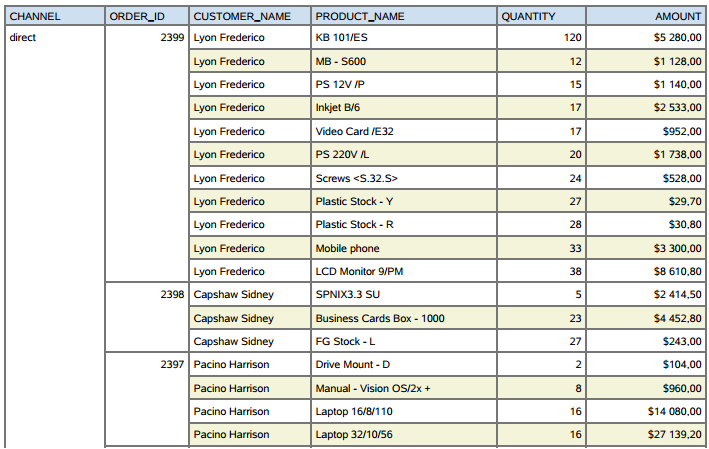
\includegraphics[scale=0.75]{master_detail_publisher}

\subsection{Raport macierzowy}
Poniżej przedstawiony jest raport macierzowy (krzyżowy) utworzony w programie Oracle XML Publisher. Zawiera informacje o zależności wydatków na pewne produkty w zależności od położenia geograficznego.

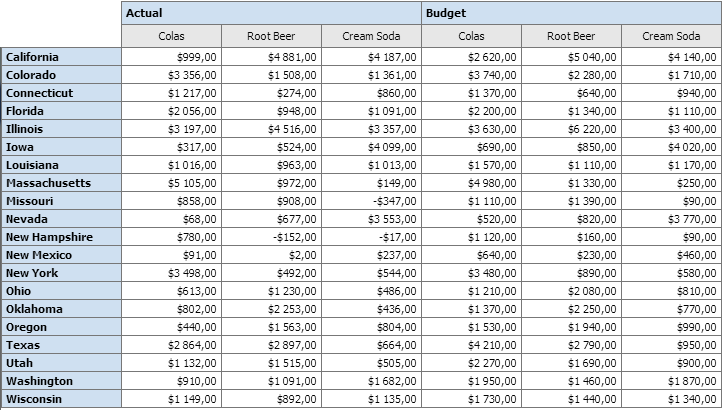
\includegraphics[scale=0.75]{crosstab_publisher}

% opis Apache FOP
\section{Apache FOP}\label{sec:fop}
Apache FOP (Formatting Objects Processor) jest programem napisanym w Javie, który konwertuje pliki zapisane w formacie XSL-FO na pliki w formacie PDF lub innych drukowalnych, m.in. RTF czy PostScript. Najnowsza stabilna wersja jest w znacznym stopniu zgodna ze specyfikacją XSL-FO 1.1. 

FOP może być wykorzystywane zarówno jako niezależna aplikacja uruchamiana np. z wiersza poleceń, jak i biblioteka Javy, dzięki czemu może być wykorzystany w każdej aplikacji tworzonej w języku Java. FOP umożliwia również przetwarzanie danych w formacie XML przy użyciu odpowiednich transformacji XSLT.

%raporty z apexa
\section{Raportowanie w ApEx}\label{sec:raporapex}
Oracle Application Express sam w sobie nie generuje raportów w formacie PDF. Aby to umożliwić, należy wykorzystać zewnętrzne narzędzie: Oracle XML (BI) Publishera, APEX Listenera lub Apache FOP uruchamianego jako serwlet na serwerze aplikacyjnym. W tej pracy zastosowana będzie tylko ostatnia metoda.

Schemat poglądowy wykorzystania FOP przez Apex'a prezentuje poniższy obrazek:

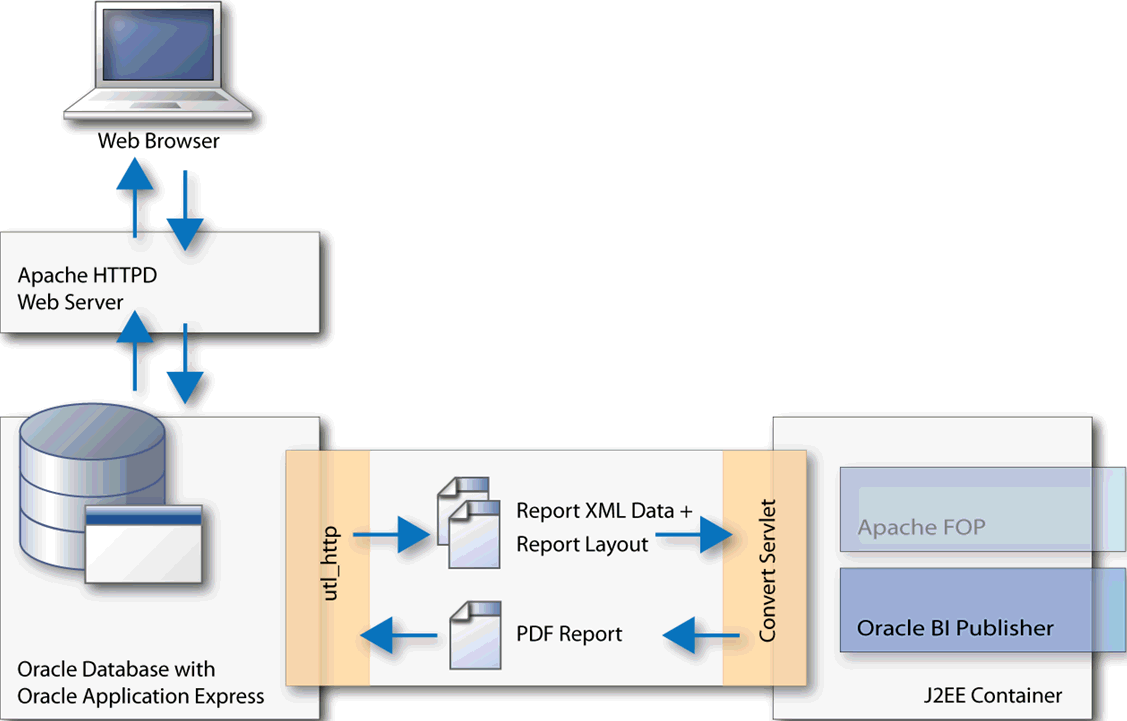
\includegraphics[scale=0.5]{apex_fop_usage}


Wersja 4.2.2 Application Express pozwala na stosowanie własnych wzorców wyglądu raportu zapisanych w XSL-FO. Istnieją darmowe narzędzia za pomocą których mozna wczytać dane w formacie XML, dostosować np. ich rozmieszczenie na stronie raportu metodą drag\&drop, a następnie wygenerować skrypt XSLT transformujący dane na wynikową stronę raportu. 

\section{Format zapisu wzorca wyglądu raportu}\label{sec:formatywzorce}
Aby możliwe było wygenerowanie raportu, niezbędny jest wzorzec ich wyglądu. Należy wybrać jakiś format spośród wielu istniejących, przy czym głównym czynnikiem jest łatwość przetwarzania i istnienie darmowych narzędzi do graficznej edycji. W związku z tym najsensowniejszym rozwiązaniem wydają się formatu bazujące na XML - SVG lub XSL-FO, a to ze względu na istnienie wielu parserów XML zgodnych ze standardami SAX i DOM. Dla obu standardów istnieją narzędzia wspomniane wcześniej - dla SVG jest to np. open source'owy SVG-edit działający w przeglądarce. Dla XSL-FO niestety trudniej znaleźć darmowe oprogramowanie, ale można wykorzystać Altova StyleVision (darmowa wersja basic w zupełności wystarczy na potrzeby tej pracy). 

Ostatecznie jako wzorzec zostanie wykorzystany format XSL-FO.



 
\end{document}